\section{Deterministic Adaptation and Other Means of Performance Improvement}
\label{s:optimizations}

A key insight behind the performance of \lib{} is that deterministic execution does not preclude adaptation on the part of the runtime system. 
Philosophically, a program running under varying conditions cannot be fully deterministic: while the output may be completely deterministic, the time to completion generally is not.
Accordingly, we may adapt to the behavior of the running program, as long as the determinism of program state is preserved. 

In principle, a great number of changes to the underlying execution environment are possible without affecting determinism, either in response to environmental changes or in response to (deterministic) program behaviors. Below, we discuss two such adaptations, followed by three other optimizations used in \lib{}.

%\subsection{Thread Reuse for Fork-Join Programs}
%
%In order to support fork-join programs it is imperative for \lib{} to provide fast thread creation and tear-down. However, the use of processes with private heap and globals segments makes this a challenging goal. When a program invokes \create{}, it effectively forks a new process, and each populated \pte{} in the heap and globals segments must be copied into the child's page table. This can be a large number of entries to copy and adds a significant amount of latency to thread creation. 
%
%To mitigate this effect, we can reuse existing threads that have exited previously during the program. When a thread invokes \create{}, it first checks to see if a thread is waiting in the thread pool. If the pool is empty, a call to \fork{} is initiated; otherwise a thread from the pool is chosen. We prefer to chose a thread that has recently exited over an older thread. The reason for this is that a recently exited thread will have a more recent working copy and thus will require less work by \update{} upon startup. 
%
%Because the stack is not \conversion{}-enabled, a thread taken from the pool will have a stale view of the stack segment. Thus, in order to support stack-allocated arguments to threads, we take a snapshot of the parent's stack and copy it into the child on startup. 


\subsection{Adaptive Coarsening}

\begin{figure*}[t]
\centering
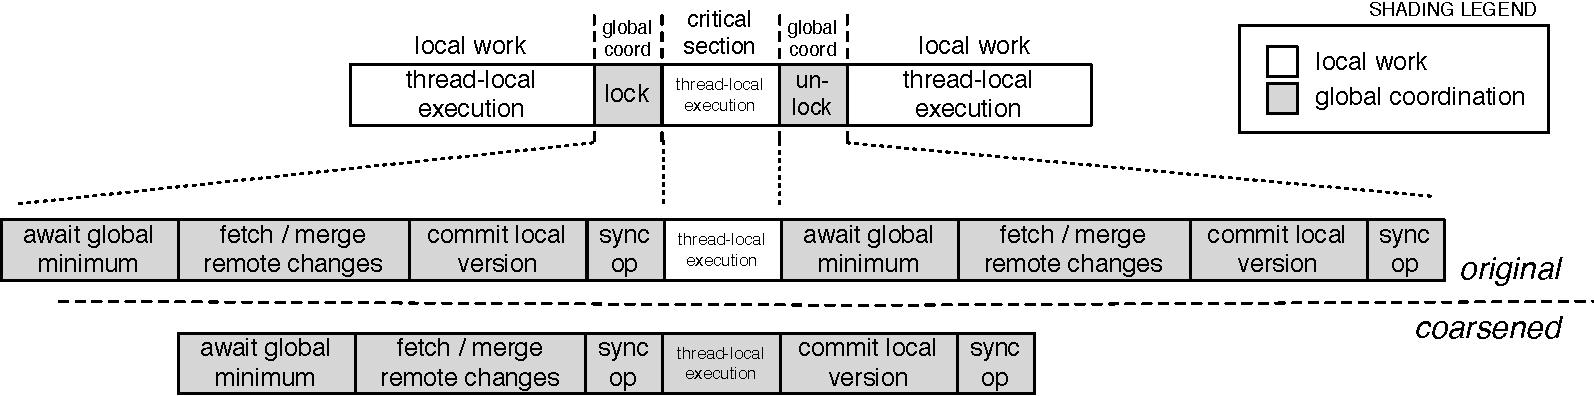
\includegraphics[width=6.8in]{figures/coarsening}
\caption{Program execution under \lib{} is divided into phases of local work and global coordination. In this example, a critical section is surrounded by two phases of global coordination, for the lock and unlock operations respectively. The lower part of the figure shows the result of coarsening on this example.}
\label{f:coarsening}
\end{figure*}

Fig. \ref{f:coarsening} illustrates the operation of \lib{} for a critical section. In the local work phase, all changes are made to the local copy. When a synchronization operation is reached, the thread enters the global coordination phase. It sleeps until it has the global minimum instruction count (GMIC) and can acquire the token, then retrieves any remote updates, and commits its own changes before acquiring the lock. It then releases the token and begins its critical section. The critical section constitutes another local work chunk, which is followed by another global coordination phase. 

From this example, it is clear that though the work performed in the global coordination phase may be highly optimized, each deterministic synchronization operation will incur substantial overhead vs. its nondeterministic equivalent. This problem becomes particularly severe when the time between synchronization operations is brief, such that the local work is dwarfed by the global coordination surrounding it. 

To address this problem, we propose to adaptively reduce the number of global coordination phases, through a technique we call coarsening. In essence, coarsening combines several global coordination phases into a single phase, which includes the intervening local work chunks. The lower part of Fig. \ref{f:coarsening} illustrates the effect of coarsening on a single critical section. Here, the coordination work required is substantially reduced, at the cost of moving what used to be (parallel) local work into the (serialized) global coordination phase. 
As discussed in more detail below, coarsening is not limited to pairs---any number of local work chunks and their surrounding coordination may be coarsened into a single, longer global coordination phase. 

%Recall that a {\it chunk} is a unit of local work that appears between global synchronization phases. 
%When the chunk length is short, the cost of a \lib{} memory fence can become the dominating factor in program execution time. Each memory fence must read the performance counter, wait until its DLC is the global minimum, acquire/release the token and invoke \conversion{} to commit/update/merge memory. For this reason, short chunks can create a significant amount of sequential overhead.

%\TODO{this reads as if we're doing coarsening for everything, but in fact the only coarsening candidates are lock and unlock}

%We can reduce the number of memory fences by coarsening the chunks, creating longer chunk lengths that can effectively mask the overhead of a fence. 
While this technique sounds straightforward, several challenges arise. First, in order to maintain TSO consistency, other threads are blocked at their next synchronization operation until the coarsened chunk has completed. This means that an overly ambitious coarsening policy, producing excessively long coarsened chunks, can significantly harm the overall system by causing excessive waiting of other threads. Second, the choice of when to begin a coarsened chunk must be an informed one. If \lib{} chooses to coarsen and the next chunk is very long (which cannot be known ahead of time) the result would be a net loss in performance. Finally, these decisions need to be done deterministically.

Our approach is to use an adaptive coarsening policy that estimates, for each synchronization variable, the next chunk length using an exponentially weighted moving average of earlier chunk lengths. One such estimate is maintained per lock, for use with coarsening $lock$ operations, and a thread-local estimate is maintained for use with coarsening $unlock$ operations.  
%On completion of a chunk we add the length to a thread-local exponentially weighted moving average (EWMA). Before we execute a memory fence and begin the next chunk we consult the EWMA for a guess of what the next chunk length will be. 
Coarsening proceeds until either (a) the estimated total coarsened chunk length exceeds a maximum threshold, or (b) a conditional variable or barrier operation is encountered. 
%If $current\_length+chunk\_length\_estimate < max\_coarsening\_length$ then we will elide the memory fence and continue. 
%For more accurate statistics we use the synchronization variable as additional context by storing per-variable EWMA's. 

We deterministically adapt the maximum chunk length at runtime, using a multiplicative increase, multiplicative decrease policy. 
Each time a thread $T1$ enters the global coordination phase, $T1$ compares its thread id to the id of the thread $T2$ that previously entered the global coordination phase.
If $T1==T2$, the maximum chunk length is doubled. Conversely, if $T1\neq{}T2$, the maximum chunk length is halved. 
This allows each thread to individually adapt to current conditions.
Because all decisions are based on chunk lengths and the token order, both of which are deterministic, coarsening maintains determinism.

\subsection{Adaptive Counter Overflows}

A thread's logical clock can be updated primarily in one of two ways: (1) when a thread finishes a chunk and the performance counter is read and (2) when a performance counter overflows, triggering an interrupt. Regarding the latter, the choice of overflow frequency is a trade-off between sequential overhead and logical clock accuracy. With a low frequency of overflows, a thread that is not the GMIC may wait longer to receive the notification that they are the new global minimum. However, if the frequency is too high, the cost of exception handling can become unwieldy (see \cite{olszewski_kendo:_2009} for further discussion). 

Our solution to this problem is based on the observation that overflow frequency does not impact determinism at all. A lower or higher frequency may impact when a thread is notified in real time, but it has no bearing in logical time. Therefore,  we design our logical clock module to adapt our overflow frequency using three simple rules. First, at the beginning of each chunk, the overflow is set to a conservative base value of 5,000 retired instructions. Second, if we are the GMIC, then at the beginning of each chunk and at each overflow we check to see if the next lowest logical clock is currently waiting to become the GMIC. If so, we set the performance counter to overflow just when our clock exceeds theirs. Third, if there is not a thread that we must notify then we double the number of instructions that will occur before the next overflow. 

%\subsection{Other Optimizations}

\subsection{Thread Reuse for Fork-Join Programs}

In order to support fork-join concurrency it is imperative for \lib{} to provide fast thread creation and tear-down. However, the use of processes with \conversion{} memory makes this a challenging goal. When a new thread is spawned the call is intercepted by \lib{} and instead a new process is forked (\S\ref{s:isolation}). Because \conversion{} memory is mapped as a private segment, each populated page-table entry in the \conversion{} segment must be copied into the child's page-table. Depending on the application, this can be a large number of entries to copy and adds a significant amount of latency to thread creation. To help mitigate this issue, \lib{} keeps a pool of threads that have recently finished executing. When spawning a new thread, if a thread is waiting in the pool that thread is reused, eliminating an expensive fork operation. The newly spawned thread will still have to update its view of memory to reflect what has been committed since it began waiting in the pool. However, this is typically a much cheaper operation than forking a new process.

\subsection{User Space Reading of Performance Counters}

Our deterministic logical clock module resides primarily in the kernel. One advantage of this approach is that performance counter overflows that identify a new GMIC can notify waiting threads directly from kernel space using shared memory, avoiding costly signals to user space for each overflow. There is added cost to this design however, as \lib{} would require system calls at the end of each chunk to read the counters and determine (and potentially notify) a newly-appointed GMIC thread. To avoid the system call latency for short chunks, we allow user space reading of the performance counters when executing a coarsened chunk.

\lstset{numbers=left,language=C, basicstyle={\footnotesize\ttfamily},tabsize=1,frame=shadowbox,linewidth=7cm,numbers=left}

\newsavebox{\mutexLock}
\begin{lrbox}{\mutexLock}% Store first listing
\begin{lstlisting}
void mutexLock(lock_t* l){
	clockPause();
	while(true){
		waitToken();
		if (lockAcq(l)){;
			convCommitAndUpdateMem();
			break;
		}
		else{
			clockDepart();
			insert(l->waitQueue, _tid);
			releaseToken();
			waitForRelease(l);
		}
	}
	releaseToken();
	clockResume();
}
\end{lstlisting}
\end{lrbox}


\newsavebox{\waitToken}
\begin{lrbox}{\waitToken}% Store first listing
\begin{lstlisting}
void waitToken(){
	while(!isGMIC() || token!=NULL){}
	token=_tid;
}

void releaseToken(){
	token=NULL;
}
\end{lstlisting}
\end{lrbox}

\begin{figure}
\hspace*{.5cm}
\usebox{\mutexLock}
\caption{mutexLock() implementation.}
\label{f:mutexLock}
\end{figure}


\begin{figure}
\hspace*{.5cm}
\usebox{\waitToken}
\caption{A simplified implementation of token acquisition and release.}
\label{f:waitToken}
\end{figure}


\subsection{Fast Forward}
\label{s:fast-forward}

A thread may wait on a conditional variable or lock for an indefinite amount of time, causing its logical clock to become further and further behind the rest of the threads in the system. When the thread is finally woken and acquires the token, it may be the GMIC thread for a long time to come. To combat this, \lib{} ``fast forwards'' a thread's logical clock to the value of the logical clock of the last thread to release the token if that thread had a larger clock.\footnote{Kendo \cite{olszewski_kendo:_2009} employed a similar mechanism to avoid excessive logical clock increments in their locking algorithm.} 

%%% Local Variables: 
%%% mode: latex
%%% TeX-master: "paper.tex"
%%% End:
